\documentclass[a4paper,11pt]{article}
\usepackage[utf8]{inputenc}
\usepackage[T1]{fontenc}
\usepackage[swedish]{babel}
\usepackage{amsmath,amssymb,amsfonts}
\usepackage{tikz}
\usepackage{pgfplots} % För snygga och flexibla grafer
\pgfplotsset{compat=1.17} % Anpassa version vid behov
\usepackage{enumitem}
\usepackage{geometry}
\geometry{margin=2.5cm}

\title{Prövning Matematik 1b}
\author{Partille Gymnasium}
\date{29 augusti 2025}

\begin{document}

\maketitle

\begin{center}
\fbox{\parbox{0.93\textwidth}{
\textbf{Information och regler:}\\
\vspace{2mm}
\begin{itemize}[leftmargin=*,nosep]
    \item Du \textbf{får använda} miniräknare, linjal och formelblad.
    \vspace{2mm}
    \item Mobiltelefoner och andra kommunikationsmedel är \textbf{inte tillåtna}.
    \vspace{2mm}
    \item Tystnad gäller i provsalen.
    \vspace{2mm}
    \item Svara tydligt och visa alla uträkningar på ett \textbf{separat papper}.
    \vspace{2mm}
    \item Provet består av \textbf{två delar}, men samma regler gäller för bägge delarna.
    \vspace{2mm}
    \item \textbf{Inga toabesök}, utom mellan delarna. Du får då inte tillbaka din första del.
    \vspace{2mm}
    \item Misstänkt fusk kommer resultera i att provet inte kan bedömmas.
\end{itemize}
\vspace{2mm}
}}
\end{center}

\begin{center}
\fbox{\parbox{0.93\textwidth}{
Jag skriver under på att jag tagit del av reglerna ovan och följer dem:

\vspace{2mm}
\textbf{Namn:}\hrulefill\hspace{1cm}\textbf{Klass:}\hrulefill
}}
\end{center}

\newpage

\section*{Del A}
\begin{enumerate}[label=\textbf{\arabic*.}]
    % Algebra och ekvationer
    \item Lös ekvationen: $2x + 5 = 19$
    \item Förenkla uttrycket: $4a - 2(a + 3)$
    \item Nedan visas grafen till en funktion $f(x)$. Svara på frågorna:
    \begin{enumerate}[label=\alph*)]
        \item Bestäm $f(2)$ med hjälp av grafen.
        \item Lös ekvationen $f(x) = 3$ med hjälp av grafen.
    \end{enumerate}
    \begin{center}
    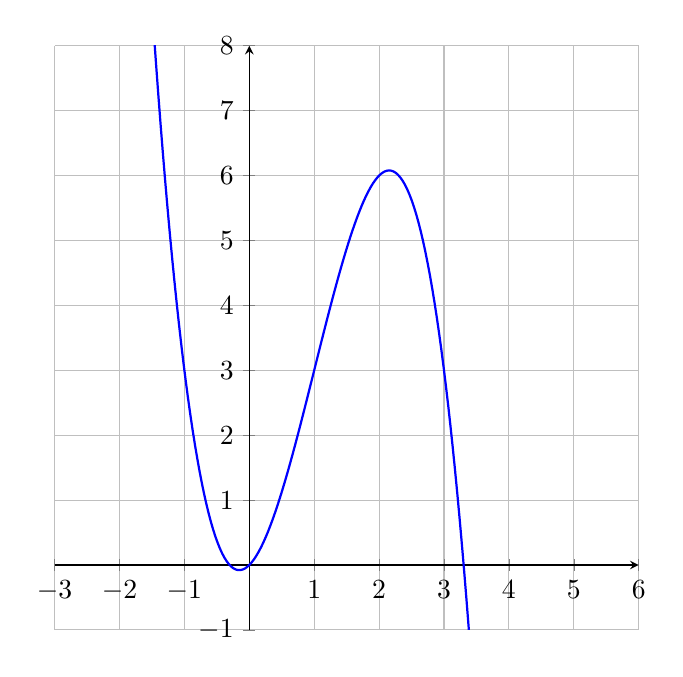
\begin{tikzpicture}
      \begin{axis}[
        axis lines=middle,
        axis line style/.append style={-},
        grid=both,
        xmin=-3, xmax=6,
        ymin=-1, ymax=8,
        samples=200,
        width=9cm,
        height=9cm,
        domain=-2:5,
        xtick distance=1,
        ytick distance=1,
        clip=true
      ]
        \addplot[blue, thick] {-x^3 + 3*x^2 + x };
      \end{axis}
    \end{tikzpicture}
    \end{center}
    \item En linjes ekvation skrivs: $y = 2x - 5$. Vad är lutningen för linjen?
    \item En varas pris sänks med 20\%, och höjs sedan med 40\%. 
    \begin{enumerate}[label=\alph*)]
      \item Vad blir den totala procentuella förändringen?
      \item Vad blir den totala förändringsfaktorn?
    \end{enumerate}
    \item Ett banklån på 36000 kronor ska amorteras med samma belopp varje månad på 5 år. Hur mycket ska amorteras varje månad?
    \item Förenkla uttrycket: $\displaystyle \frac{2^5 \cdot 2^{-2}}{2^3}$
    \item En person sätter in 5000 kr på ett konto med 4\% ränta per år. Hur mycket pengar har personen efter 6 år om räntan räknas på hela beloppet varje år?
  
\newpage
    \item Nedan visas grafen till en linjär funktion.
    \begin{enumerate}[label=\alph*)]
        \item Vad är lutningen för linjen?
        \item Bestäm linjens ekvation på formen $y = kx + m$.
    \end{enumerate}
    \begin{center}
    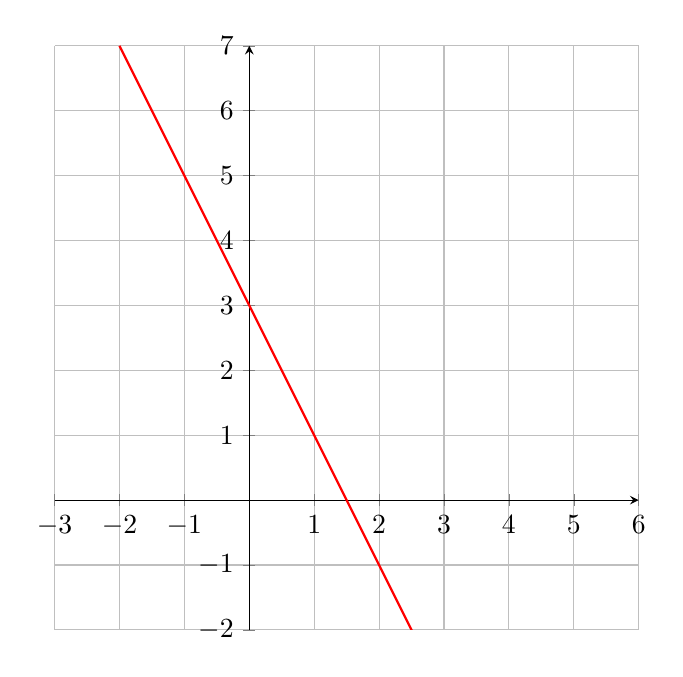
\begin{tikzpicture}
      \begin{axis}[
        axis lines=middle,
        axis line style/.append style={-},
        grid=both,
        xmin=-3, xmax=6,
        ymin=-2, ymax=7,
        samples=200,
        width=9cm,
        height=9cm,
        domain=-2:5,
        xtick distance=1,
        ytick distance=1,
        clip=true
      ]
        \addplot[red, thick] {-2*x + 3 };
      \end{axis}
    \end{tikzpicture}
    \end{center}
    \item En enkät undersökning gjordes på Partille Gymnasium där de undersökte om kvalitén på skolmaten blivit sämre. 
    \\ \\Totalt frågades 292 elever.
    \\ \\120 elever svarade \textbf{ja}.
    \\ \\92 elever svarade \textbf{nej}.
    \\ \\Utifrån enkäten
    \begin{enumerate}[label=\alph*)]
      \item Hur stor andel av eleverna svarade ja?
      \item Hur stor andel av eleverna svarade nej?
      \item Hur många elever svarade inte på enkäten?
      \item Om vi tar hänsyn till bortfallet, hur stor andel av eleverna skulle kunna svara nej?
      \item Kan vi statistik säkerhet påstå att majoriteten av eleverna på Partille Gymnasium tycker skolmaten blivit sämre? Motivera!
      
  \end{enumerate}
\newpage
\section*{Del B}
    \item Lös ekvationen: $\frac{3y}{2} -2 = y + 4$
    \item Faktorisera uttrycket: $6x^2y + 9xy^2$
    \item En rät linje går genom punkterna (1,2) och (4,8). Bestäm linjens ekvation på formen $y = kx + m$.
    \item I en låda finns 5 röda och 3 blå kulor. Du tar två kulor ur lådan utan att lägga tillbaka den första.
    \begin{enumerate}[label=\alph*)]
      \item Vad är sannolikheten att du tar två röda kulor?
      \item Vad är sannolikheten att du tar en röd och en blå kula?
    \end{enumerate}
    \item Nedan ser du tre grafer i samma koordinatsystem. Avgör vilken \textbf{typ av funktion} varje graf motsvarar. Motivera!
    \begin{center}
    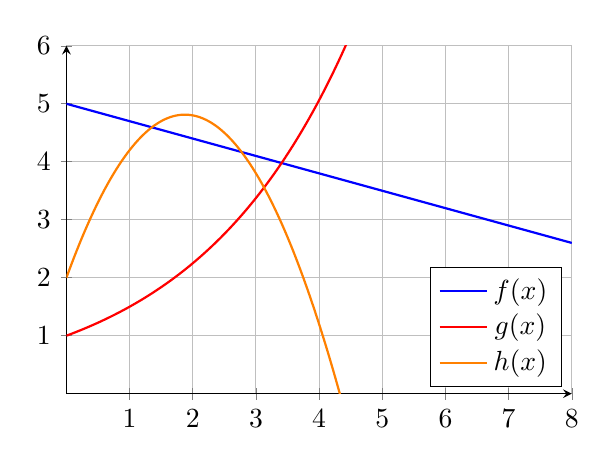
\begin{tikzpicture}
      \begin{axis}[
        axis lines=middle,
        axis line style/.append style={-},
        grid=both,
        xmin=0, xmax=8,
        ymin=0, ymax=6,
        samples=200,
        width=8cm,
        height=6cm,
        domain=0:8,
        xtick distance=1,
        ytick distance=1,
        clip=true,
        legend style={at={(0.98,0.02)},anchor=south east}
      ]
        \addplot[blue, thick] {-0.3*x+5};
        \addlegendentry{$f(x)$}
        \addplot[red, thick] {1*1.5^x};
        \addlegendentry{$g(x)$}
        \addplot[orange, thick] {-0.8*x^2+3*x+2};
        \addlegendentry{$h(x)$}
      \end{axis}
    \end{tikzpicture}
    \end{center}
    \item Viktor har köpt en begagnad mobiltelefon. Priset på telefonen kan beräknas med formeln $y=9000 \cdot 0.8^x$ där $x$ är antalet år sedan telefonen var ny.
    \begin{enumerate}[label=\alph*)]
      \item Vad kostade telefonen när den var ny?
      \item När Viktor köpte den var telefonen 3 år gammal, hur mycket betalade han för den?
      \item Hur mycket minskar priset på telefonen per år i procent?
    \end{enumerate}
    \item Ange lutningen för en linje som är parallell med linjen $2y-6x-7=0$.
    \item En taxi kostar 45 kr i startavgift och därefter 12 kr per kilometer. 
    \begin{enumerate}[label=\alph*)]
      \item Skriv en formel för totalkostnaden $K(x)$ om du åker $x$ kilometer.
      \item Använd formeln för att beräkna kostnaden för en resa som är 5 kilometer lång.
      \item Använd formeln för att beräkna hur långt du kan resa för 165 kr.
    \end{enumerate}
    \end{enumerate}
\end{document}
